\section{Data Encoding with Triplet Network}

Our proposed semi-supervised classification approach addresses a critical challenge in clustering high-dimensional data by integrating Contrastive Learning techniques \cite{Hoffer_2015,Khosla_2020} with Stochastic Quantization. While the Stochastic Quantization algorithm (\ref{sq-objective-fn-gradient:eq}) effectively mitigates scalability issues for large datasets, it remains susceptible to the "curse of dimensionality," a phenomenon common to clustering methods that rely on distance minimization (e.g., K-Means and K-Means++). Kriegel et al. \cite{Kriegel_Kröger_Zimek_2009} elucidated this phenomenon, demonstrating that the concept of distance loses its discriminative power in high-dimensional spaces. Specifically, the distinction between the nearest and farthest points becomes increasingly negligible:

\begin{equation}
    \label{dimensions-precision-ratio:eq}
    \lim_{n \to \infty} \frac{\max d(\xi_i, y_k) - \min d(\xi_i, y_k)}{\min d(\xi_i, y_k)} = 0
\end{equation}

Our study focuses on high-dimensional data in the form of partially labeled handwritten digit images \cite{lecun2010mnist}. However, it is important to note that this approach is not limited to image data and can be applied to other high-dimensional data types, such as text documents \cite{Radomirovic_2023,Widodo_2011}. While efficient dimensionality reduction algorithms like Principal Component Analysis (PCA) \cite{Abdi_Williams_2010,Deisenroth_Faisal_Ong_2020} exist, they are primarily applicable to mapping data between two continuous spaces. In contrast, our objective necessitates an algorithm that learns similarity features from discrete datasets and projects them onto a metric space where similar elements are grouped into clusters, a process known as similarity learning.

Recent research by \cite{MURASAKI_ANDO_SHIMAMURA_2022} and \cite{Turpault_Serizel_Vincent_2019} has employed a Triplet Network architecture to learn features from high-dimensional discrete image data and encode them into low-dimensional representations in the latent space. These authors proposed a semi-supervised learning approach where the Triplet Network is trained on a labeled subset of data to encode them into latent representations in $\mathbb{R}^n$, and subsequently used to project the remaining unlabeled fraction onto the same latent space. This approach significantly reduces the time and labor required for data annotation without compromising accuracy.

The Triplet Network, introduced by \cite{Hoffer_2015}, is a modification of the Contrastive Learning framework \cite{Khosla_2020}. Its core idea is to train the model using triplets of samples:

\begin{enumerate}
    \item An anchor sample $\xi_i$: a randomly sampled element from the feature set $\Xi$
    \item A positive sample $\xi^+_i$: an element with a label similar to the anchor $\xi_i$
    \item A negative sample $\xi^-_i$: an element with a label different from the anchor $\xi_i$
\end{enumerate}

Unlike traditional Contrastive Learning, which compares only positive $\xi^+_i$ and negative $\xi^-_i$ samples, the Triplet Network learns to minimize the distance between the anchor and positive samples while maximizing the distance between the anchor and negative samples. This is achieved using the triplet loss objective function (see Fig.~\ref{triplet-network:fig}):

\begin{equation}
    \label{triplet-loss-func:eq}
    \mathcal{L}_{triplet} = \max (0, d(f_{\theta}(\xi_i), f_{\theta}(\xi^+_i)) - d(f_{\theta}(\xi_i), f_{\theta}(\xi^-_i)) + \alpha)
\end{equation}

\noindent where $f_{\theta}: \Xi \to \mathbb{R}^n$ is a parameterized abstract operator mapping discrete elements $\Xi$ into latent representations (in our case, a Triplet Network with weights $\theta$), $d: [\mathbb{R}^n, \mathbb{R}^n] \to \mathbb{R}$ is a distance metric between samples, and $\alpha$ is a margin hyperparameter enforcing a minimum separation between positive and negative pairs. Analogous to the Stochastic Quantization distance metric (\ref{sq-objective-fn:eq}), we employed the Euclidean norm $l_2$ for $d(\xi_i, \xi_j)$ in (\ref{triplet-loss-func:eq}).

\begin{figure}
    \centering
    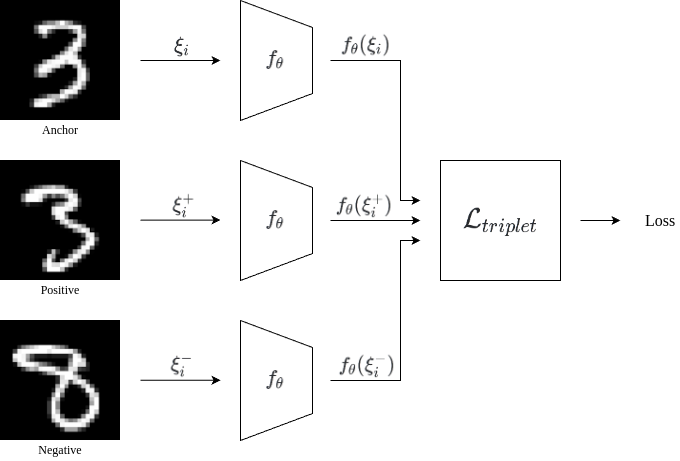
\includegraphics[width=0.75\textwidth]{figures/triplet_loss.png}
    \caption{Triplet Network structure for MNIST dataset \cite{lecun2010mnist}.} \label{triplet-network:fig}
\end{figure}

In our research, we utilized a Convolutional Network architecture as $f_{\theta}$, as proposed by \cite{Lecun_1998}. The detailed overview of the architecture, its training using the Backpropagation algorithm, and accuracy evaluation are beyond the scope of this paper; however, \cite{Beohar_2021}, \cite{Krizhevsky_2012}, and \cite{Lecun_1998} provide extensive coverage of these topics.

Regarding triplet mining strategies for $(\xi_i, \xi^+_i, \xi^-_i)$, it is crucial to select an approach that produces the most informative gradients for the objective function (\ref{triplet-loss-func:eq}). \cite{xuan2020} discusses various online triplet mining strategies, which select triplets within each batch of a training set on each iteration. We employed the semi-hard triplet mining strategy, which chooses an anchor-negative pair that is farther than the anchor-positive pair but within the margin $\alpha$:

\begin{equation}
    \label{semi-hard-triplet-mining:eq}
    \xi^-_i = \argmin_{\substack{\xi: C(\xi_i) \neq C(\xi) \\ d(f_{\theta}(\xi_i), f_{\theta}(\xi)) > d(f_{\theta}(\xi_i), f_{\theta}(\xi^+_i))}} d(f_{\theta}(\xi_i), f_{\theta}(\xi))
\end{equation}

\noindent where $C(\xi)$ denotes the label of an element $\xi$.

By applying ideas from \cite{Hoffer_2015,MURASAKI_ANDO_SHIMAMURA_2022,Turpault_Serizel_Vincent_2019}, we can utilize the encoded latent representations of the Triplet Network to train a Stochastic Quantization (\ref{sq-objective-fn-gradient:eq}) algorithm. This novel approach enables us to solve supervised or semi-supervised learning problems of classification on high-dimensional data. The semi-supervised learning process using the combined algorithm, assuming we have a labeled subset $\xi \subset \Xi$ and remaining unlabeled data $\bar{\xi} \subset \Xi, \bar{\xi} \cap \xi = \varnothing$, can be summarized as follows:

\begin{enumerate}
    \item Train a Triplet Network $f_{\theta}$ on labeled data $\xi$ and produce encoded latent representations space $\bar{\Xi} \subset \mathbb{R}^n$
    \item Utilize the trained Triplet Network $f_{\theta}$ to project the remaining unlabeled data $\bar{\xi}$ onto the same latent representation space $\bar{\Xi}$
    \item Employ both labeled and unlabeled latent representations to train a Stochastic Quantization (\ref{sq-objective-fn-gradient:eq}) algorithm
\end{enumerate}